\documentclass[manuscript,nonacm]{acmart}
\settopmatter{printacmref=false,printfolios=true}
\title{Retrieved Abstract Context and PubMedQA Accuracy: A Matched Comparison with FLAN-T5-small}
\author{Rahul Mahto}
\affiliation{\institution{Indian Institute of Information Technology Allahabad}\country{India}}
\begin{document}
\begin{abstract}
We evaluated one frozen FLAN-T5-small checkpoint on the 500 official PubMedQA test questions using three matched conditions: closed-book, TF--IDF top-1 context from a fixed 1,000-document corpus, and reference context. Accuracy was 34.6\%, 52.8\%, and 53.4\%, respectively. The primary paired gain from TF--IDF was 18.2 percentage points (95\% bootstrap interval, 11.4 to 24.8). TF--IDF recovered the paired source on 433 questions. Among 67 misses, reference context recovered 16 retrieved-context errors and reversed 13 correct predictions. All conditions scored below the always-yes benchmark and produced no maybe predictions. The results quantify label agreement and source recovery for this checkpoint and corpus.
\end{abstract}
\maketitle
\section{Introduction}
Recovering the intended source and generating a correct answer are separate outcomes. A retriever can locate the benchmark's paired abstract while the generator still disagrees with the answer label. Another abstract may contain useful information even when its identifier differs from that of the source. This distinction matters when evaluating external evidence for domain-specific research questions.

This experiment follows a review of grounded and ungrounded language models and its retrieval-only pilot \cite{mahtoReview}. The pilot compared TF--IDF, BM25, and reciprocal rank fusion on 18 exploratory test questions over 15 synthetic, source-correlated passages. The review reports that TF--IDF and rank fusion each ranked the designated passage first for 12 of the 18 questions, compared with 11 for BM25. The raw pilot execution artifacts were unavailable for independent verification \textbf{[TO VERIFY]}. No generator ran in the pilot. Its results concern evidence access and do not establish generated-answer accuracy.

We ask how much accuracy changes when a single TF--IDF result is supplied to a fixed FLAN-T5-small checkpoint, compared with an empty context slot. We also measure performance with the benchmark's paired abstract body and examine whether substituting that body on source misses changes correctness. Our contribution is a checkpoint-specific estimate on the official PubMedQA test set, with paired transitions and a separate source-recovery diagnostic.

\section{Related Work}
Lewis et al.\ combined a pretrained sequence-to-sequence generator with dense Wikipedia retrieval and evaluated knowledge-intensive tasks \cite{lewis2020}. Their work motivates testing what an external context adds to a generator. We examine a narrower intervention: a sparse lexical lookup that supplies one abstract at inference time while leaving model weights fixed.

Shuster et al.\ compared parametric and retrieval-augmented approaches for knowledge-grounded dialogue and used human ratings to assess conversational hallucination \cite{shuster2021}. Their study motivates evaluating the output separately from access to evidence. Our generator produces a categorical answer and the scoring reference is the benchmark label. There are no human judgments of factual claims or conversational quality.

Jin et al.\ introduced PubMedQA with biomedical research questions, paired abstracts with conclusions removed, separate long answers, and yes/no/maybe decisions \cite{jin2019}. The official split makes label scoring reproducible, while the paired PMID provides a source identity for retrieval evaluation. The original supervised results supply historical context. Their training conditions differ from our use of a frozen instruction-tuned generator.

Xiong et al.\ benchmarked medical retrieval-augmented generation across multiple corpora, retrievers, and backbones, including comparisons on PubMedQA \cite{xiong2024}. BioHarness reported PubMedQA comparisons with no context, retrieved evidence, and golden context using a shared backbone \cite{xiao2026}. These precedents establish that the three evidence regimes have already been studied. The present study estimates their outcomes under one small checkpoint and one fixed lexical policy.

\section{Methodology}
\subsection{Questions and candidates}
The 500 keys in the official ground-truth JSON define the test set \cite{jin2019,pqadata}. The six smoke PMIDs are the first six numerically sorted non-test keys: 1571683, 2224269, 2503176, 8017535, 8111516, and 8200238. Non-test positions seven through 26 were reserved for optional prompt checks. Whether any optional checks were executed remains unconfirmed \textbf{[TO VERIFY]}. Both sets are disjoint from the test PMIDs.

Each of the 1,000 PQA-L records contributes one document. Its released \texttt{CONTEXTS} segments are stripped, empty segments are discarded, and the remainder are joined in order with newlines. The index excludes article title metadata, question fields, long answers, and decision labels. Only the current question is used as query text. The paired test abstract bodies are deliberately present so source recovery is possible. Fitting IDF on this fixed corpus uses document text without outcome labels. Gold labels are joined by PMID after prediction export.

\subsection{Retrieval and matched input}
We fit a sparse float64 TF--IDF index over contexts ordered by numeric PMID. The representation uses lowercased word unigrams of at least two word characters, no accent stripping, no stop list, minimum document frequency one, maximum document frequency 1.0, no feature limit, natural term frequency, smoothed IDF, and $\ell_2$ normalization. Ranking uses cosine similarity. The highest positive score wins, and exact ties select the smallest numeric PMID. An all-zero query supplies an empty context and counts as a miss.

\begin{table}[htbp]
\caption{Matched conditions. The same instruction and question precede the context slot.}
\label{tab:arms}
\centering
\begin{tabular}{@{}lll@{}}
\toprule Arm & Condition & Context slot\\\midrule
A & Closed-book & Empty string\\
B & TF--IDF top-1 & Highest positive match, else empty\\
C & Reference & Paired PQA-L body by PMID\\\bottomrule
\end{tabular}
\end{table}

The instruction asks for exactly one label: yes, no, or maybe. The exact prompt is recorded in the manifest. The shared prefix contains this instruction, the exact question, and the context heading. Prefix and context are tokenized separately without special tokens. Input assembly preserves the full prefix, takes leading evidence tokens only up to the remaining budget, and appends one T5 end-of-sequence token. The 512-token cap includes this token. Identical evidence normalization in B and C means that a source hit should yield identical model inputs.

\begin{figure}[htbp]
\centering
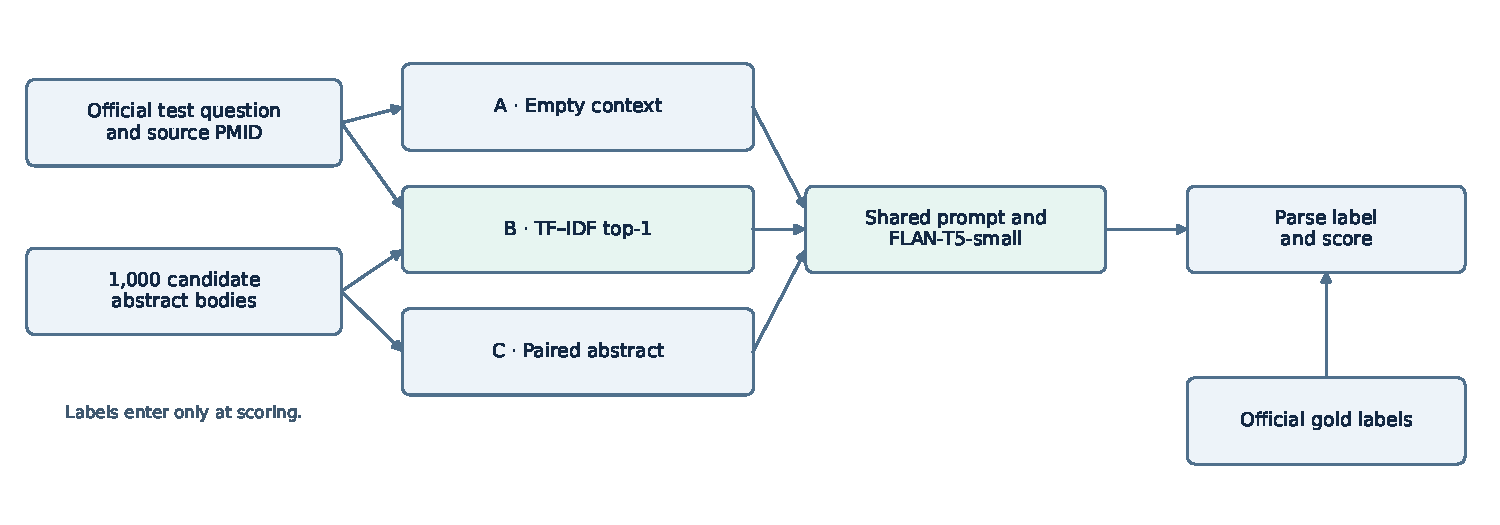
\includegraphics[width=\linewidth]{figures/pubmedqa-architecture.pdf}
\Description{The official question and candidate abstracts define three context paths. Empty context, lexical top-one context, and paired reference context enter one shared FLAN-T5-small model. Official gold labels are joined at scoring.}
\caption{Comparison pipeline. Each arm receives the same question and instruction. Arm B selects a context by lexical similarity, and arm C looks up the paired source by PMID. Official gold labels enter at scoring.}
\label{fig:architecture}
\end{figure}

\subsection{Scoring and uncertainty}
For question $i$ and condition $a$, $Y_{ia}=1$ when the parsed category agrees with the gold label and $0$ otherwise. The parser trims whitespace, lowercases, removes at most one terminal period, question mark, or exclamation mark, and trims again. Only yes, no, and maybe are accepted. Invalid outputs count as incorrect and remain in the denominator. Macro-F1 averages the three class F1 scores with zero for undefined scores. Hit@1 separately measures exact equality of the top retrieved PMID and the benchmark source PMID.

The primary contrast is $100\,\overline{(Y_{iB}-Y_{iA})}$ percentage points. We count wrong-to-right and right-to-wrong changes on the same questions. The 95\% paired percentile interval uses 10,000 resamples of 500 question indices with NumPy's default generator and seed 2026. Secondary contrasts involving C and the stratified comparisons are descriptive. On misses, reference recovery divides the number of B errors corrected by C by the number of B errors in that stratum.

\section{Experimental Setup}
\subsection{Checkpoint and environment}
The model and tokenizer are Google FLAN-T5-small \cite{chung2024,flanweights}, revision \texttt{0fc9ddf78a1e988dac52e2dac162b0ede4fd74ab}. The run manifest records CPU float32 inference, batch size one, greedy decoding, one beam, and at most eight new tokens. Sampling was disabled. Recorded versions include Python 3.13.18, PyTorch 2.14.1+cpu, Transformers 5.22.1, scikit-learn 1.6.1, and NumPy 2.4.6. The prompt, checkpoint, dataset SHA-256 hashes, ordered split IDs, and retrieval and inference settings are in \texttt{manifest.json}.

\subsection{Validation and evidence trail}
The smoke debugging log records two Colab compatibility failures. Accessing a private checkpoint attribute failed after weight loading. The proposed repair used the pinned Hub snapshot path, although the exact final loading cell remains unavailable \textbf{[TO VERIFY]}. An unavailable tokenizer assembly method was replaced by reserving space for EOS and appending it directly. The screenshots show successful ranking, tie-breaking, zero-score, truncation, label parsing, and shuffled-PMID scoring checks after the fix. They also show 18 paired smoke outputs, repeat inference, and forced hit and zero-score consistency checks. Five of the six smoke queries recovered the source, with zero natural all-zero queries. Those six questions served as engineering checks.

The reviewed notebook predates the Colab edits. The exact executed notebook and full console transcript remain pending \textbf{[TO VERIFY]}. The final run is preserved as \texttt{test-b9a5965fbf.zip}, containing 1,500 unique PMID--arm rows, pre-scoring and scored exports, the manifest, and computed tables. The post-run audit verified official PMIDs and labels, rebuilt the TF--IDF rankings, checked question and context hashes, and recomputed scores from saved outputs. It did not rerun model inference.

\section{Results}
\subsection{Overall results and paired contrasts}
\begin{table}[htbp]
\caption{Official test results from the scored predictions and arm metrics exports.}
\label{tab:overall}
\centering
\begin{tabular}{@{}lrrrrr@{}}
\toprule Condition & Questions & Correct & Accuracy & Macro-F1 & Invalid rate\\\midrule
Closed-book & 500 & 173 & 34.6\% & 0.179 & 0.0\%\\
TF--IDF top-1 & 500 & 264 & 52.8\% & 0.343 & 0.0\%\\
Reference & 500 & 267 & 53.4\% & 0.337 & 0.0\%\\\bottomrule
\end{tabular}
\end{table}

TF--IDF increased accuracy by 18.2 percentage points (95\% paired bootstrap interval 11.4 to 24.8). This comprises 200 wrong-to-right and 109 right-to-wrong transitions. Reference context scored 18.8 points above A and 0.6 points above B (descriptive, \texttt{paired\_changes.csv}). B produced the highest macro-F1 (Table~\ref{tab:overall}). The gold labels contain 276 yes, 169 no, and 55 maybe instances. An always-yes rule therefore yields 55.2\% accuracy, above all three conditions. The confusion matrices show that none of the arms predicted maybe.

\begin{figure}[htbp]
\centering
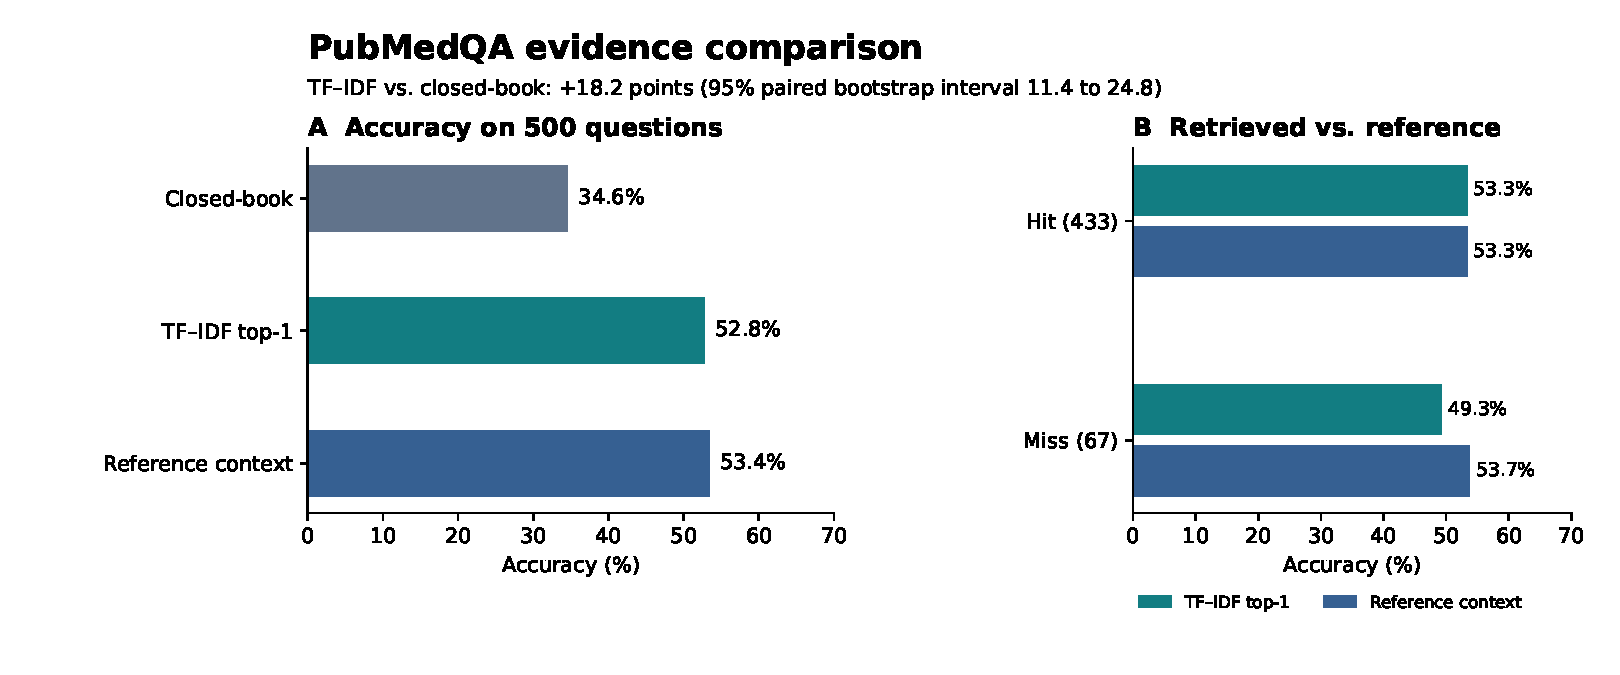
\includegraphics[width=\linewidth]{figures/pubmedqa-results.pdf}
\Description{Two horizontal bar panels. Overall accuracy is 34.6 percent closed-book, 52.8 percent with TF--IDF, and 53.4 percent with reference context. Retrieved and reference accuracies are both 53.3 percent on source hits and 49.3 and 53.7 percent on source misses.}
\caption{Accuracy by condition and exact source recovery, regenerated from saved predictions. The interval summarizes the paired B--A contrast.}
\label{fig:results}
\end{figure}

\subsection{Source hits and misses}
\begin{table}[htbp]
\caption{Accuracy by retrieval outcome from \texttt{hit\_miss.csv} and \texttt{scored\_predictions.csv}.}
\label{tab:hits}
\centering
\begin{tabular}{@{}lrrrr@{}}
\toprule Stratum & Questions & Closed-book & TF--IDF top-1 & Reference\\\midrule
Hit & 433 & 151/433 (34.9\%) & 231/433 (53.3\%) & 231/433 (53.3\%)\\
Miss & 67 & 22/67 (32.8\%) & 33/67 (49.3\%) & 36/67 (53.7\%)\\\bottomrule
\end{tabular}
\end{table}

Hit@1 was 433/500 (86.6\%), with zero all-zero queries (\texttt{retrieval\_diagnostics.csv}). All 433 hits had identical logged input-token hashes and parsed predictions for B and C. On misses, reference context recovered 16 of B's 34 errors (47.1\%) and reversed 13 correct B predictions. The resulting net gain was three correct answers, or approximately 4.5 points on the 67 misses. Figure~\ref{fig:results} shows the stratified results and Table~\ref{tab:hits} gives denominators.

\subsection{Recorded cases}
The case rule selects the smallest numeric question PMID in each category: a miss corrected by C, a miss where C reversed a correct B answer, and a hit where C was incorrect. Selections and labels come from \texttt{scored\_predictions.csv}. The reference PMID equals the question PMID.

\begin{table}[htbp]
\caption{Recorded case selections and parsed labels.}
\label{tab:cases}
\centering
\begin{tabular}{@{}llllll@{}}
\toprule Question PMID & Retrieved PMID & Gold & A & B & C\\\midrule
12098035 & 21459725 & yes & no & no & yes\\
7482275 & 24270957 & no & no & no & yes\\
7860319 & 7860319 & yes & no & no & no\\\bottomrule
\end{tabular}
\end{table}

PMID 12098035 illustrates recovery after substituting the paired source. PMID 7482275 illustrates a reversal under the same evidence substitution. PMID 7860319 illustrates a shared error despite source recovery. These records establish the label transitions and source identities. They do not identify which parts of each abstract contributed to the prediction.

\section{Discussion}
Adding a retrieved abstract raised label agreement for this checkpoint and setup. The mean gain reflects substantial bidirectional changes: the 91 net corrections arise from 200 recoveries and 109 reversals. Accuracy remains below an always-yes rule. Macro-F1 and the absence of maybe predictions expose a weakness that the invalid rate cannot capture. All outputs met the formatting rule while none assigned an example to the third category.

The reference arm probes the outcome when source selection is supplied by the benchmark. Equal predictions on hits follow from matching inputs. On misses, almost half the B errors were recovered, but the 13 reversals substantially offset the recoveries. A different source can provide useful evidence, or a prediction can agree with the benchmark for reasons unrelated to the abstract. Context clipping, ambiguous findings, and imperfect interpretation are possible explanations for individual errors. The saved outputs do not adjudicate these possibilities.

The paired setup compares a change to the context input as a whole. It does not isolate evidence relevance from length or explain the generator's internal behavior. Reporting 86.6\% source recovery alongside 53.3\% accuracy within the hit stratum preserves the distinction that motivated the transition from the pilot to the current experiment.

\section{Limitations}
The 1,000-document pool deliberately contains test sources. Title-derived questions may have strong lexical overlap with their abstract bodies. These choices constrain generalization to open PubMed search. Source-PMID identity is a narrow relevance proxy, and the hit and miss strata can differ in question difficulty and class composition. The context cap clipped 33 B contexts and 30 C contexts (\texttt{predictions.csv}). The experiment does not estimate how those cases would behave with longer input.

The pinned checkpoint identifies the evaluated model. Item-level overlap between PubMedQA and its training data remains unknown \textbf{[TO VERIFY]}. One small model, one prompt, and one sparse retrieval policy limit generalization across models and retrieval designs. The paired interval reflects question resampling, without variability from training or selecting another prompt, corpus, or checkpoint. Accuracy represents agreement with yes/no/maybe benchmark labels. Claim support, citation accuracy, and hallucination frequency were outside the measured outcomes.

\section{Conclusion}
For the frozen FLAN-T5-small checkpoint, TF--IDF top-1 context raised PubMedQA accuracy from 34.6\% to 52.8\%. Reference context reached 53.4\%. The paired analysis shows both recoveries and reversals after context changes, including on source misses. Performance remained below an always-yes rule and no condition predicted maybe. Examining label accuracy, paired errors, and source recovery together describes both the gains and the remaining weaknesses of the fixed-corpus comparison.
\section{Reproducibility and Output Mapping}
The artifact sequence has three stages. The notebook first verifies the data-file fingerprints and constructs the split and context index. Its smoke mode uses the six non-test questions to exercise generation, input assembly, and label parsing. Full mode evaluates 500 question triples and saves the raw prediction export before the evaluator joins benchmark labels. The final execution environment is reported in the manifest, including package versions and checkpoint revision. An exact rerun requires the executed Colab notebook and its compatibility edits.

\begin{table}[htbp]
\caption{Mapping between claims in this paper and files in the final run archive.}
\centering
\begin{tabular}{@{}lp{.51\linewidth}@{}}
\toprule
Archive member & Evidence\\
\midrule
\texttt{manifest.json} & Model and data pins, split identities, and run settings\\
\texttt{predictions.csv} & Raw generations and input, retrieval, and timing audit fields\\
\texttt{scored\_predictions.csv} & Gold-label join, correctness, and reproducible case selection\\
\texttt{arm\_metrics.csv}, \texttt{confusion\_*.csv} & Aggregate scores and class-level prediction counts\\
\texttt{paired\_changes.csv} & Paired transition counts and primary uncertainty interval\\
\texttt{retrieval\_diagnostics.csv}, \texttt{hit\_miss.csv} & Source recovery, stratified accuracy, and reference recoveries\\
\bottomrule
\end{tabular}
\end{table}

The saved records allow independent recomputation using the PMID as the pairing key. The scoring audit checks the raw-to-parsed mapping, recomputes per-arm summaries, and then aligns the three correctness indicators for every question. Source hits are calculated from the B-arm retrieved identifier before stratifying the matched triples. Agreement of the B and C input-token hashes on hits checks that a shared source passed through the same input construction. The exports preserve hashes and token counts, so this audit can compare logged inputs and verify the budget but cannot recover every encoded input directly.

\clearpage
\bibliographystyle{ACM-Reference-Format}
\bibliography{references}
\end{document}
